\documentclass[a4paper,3p,sort&compress]{elsarticle}

\usepackage[draft]{hyperref}
\usepackage{url}
\usepackage{booktabs}
\usepackage{graphicx}
\usepackage{xspace}
\usepackage{booktabs}
\usepackage[draft,inline,nomargin]{fixme}
\usepackage{makecell}
\usepackage{lineno}
\usepackage{natbib}
\usepackage{amsmath}
\DeclareRobustCommand{\citeext}[1]{\citeauthor{#1}~\cite{#1}}

\journal{-}

%% `Elsevier LaTeX' style
\bibliographystyle{plain}
%%%%%%%%%%%%%%%%%%%%%%%

\begin{document}
\linenumbers

% Macro para escribir NO$_2$
\newcommand{\no}{NO\textsubscript{2}\xspace}

\begin{frontmatter}

  \title{Dicrete uncertainty visualization for no levels time series forecast}


  \author{Sebasti\'an P\'erez Vasseur}
  \author{Jos\'e L. Aznarte}
  \address{Artificial Intelligence Department\\Universidad Nacional de
    Educaci\'on a Distancia --- UNED\\c/ Juan del Rosal, 16, Madrid, Spain}
  \ead{jlaznarte@dia.uned.es}
  

\begin{abstract}
  
\end{abstract}

\begin{keyword}
probabilistic forecasting \sep visualization \sep dotplot
\end{keyword}

\end{frontmatter}

%\linenumbers

\section{Introduction}
\label{sec:intro}

Hothorn \emph{et al.} stated that the real
objective in a machine learning regression analysis is to find the full conditional distribution
of the target variable. Currently, many machine learning models today only provide a point distribution, which is usually the predicted
mean of the target variable. Then the users of the model must take a decision based on the value predicted. However, only point information without uncertainty creates a false sense of deterministic result that can lead to false confidence in the decision. That's why as noted by Fernandez et Al., uncertainty improves decision making. However, users rely on visual tools and the typical visualization tools are not suited for probabilistic information, those visual tools are adapted to deterministic information.

There have been several workarounds around such issue. The first approach is to complement the point information with uncertainty. The first example that comes to our mind is the error bars in the bar chart. However, Kai et Al. showed that the information has to be intrinsic to the visualization and offered better alternatives. 

The PDF function provides a full picture of the probability. Same goes for the CDF function. However, as Fernandez et Al. states, the lack of statistical knowledge of some users deter from using those functions.  
Users can rely on less data to understand the uncertainty: Stripplots provide deciles of the target variable and the box plot provides the mean and the quantiles. This is the reason why they are more used than the pdf or cdf functions.

Also Kai et Al. investigation noted that users prefer to think in terms of natural frecuencies (2/10) instead of probabilities (.2), and therefore it's better to use discrete outcomes to communicate probabilities. cite1 cite2 used a novel visualization chart called quantile dotplot and they obtained better interpretation results using this chart to communicate uncertainty.

Quantile dotplots are built from the PDF as we can see in figure .. Then instead of using area to calculate the probability, we count the number of dots in the desired range.

\section{Time Series probabilistic charts}
\label{sec:time_series}

Time series data could also have uncertainty and they have usually been represented in 3 main types of charts: gradient, interval and box plot. Gradient time series charts uses color to represent the percentiles, however as noted by (get ref) color is a bad visual encoding to show value as users have problems to see the value it is encoded.
Interval only shows the low and bottom quantile (usually 5\% and 95\%) and lacks information that the user would have to imagine. For symwtrical pdf, it can be useful, but non symwtrical are not shown.
Finally, EPS diagrams show the range and some quantile as a box plot would do.

All those visualizations have a problem, they either encode with a bad encoding the values or have missing information quantiles. 
Many times the objective is to calculate the probability that the value will be in a certain range for a certain hour.
We propose a novel visualization technique to show the Data, that is as well discrete. We will call it time series dot plot. I'm time series dotplots, we build a stripplot for each hour, but then we use a dot instead of a bar. This way we can count the probability of a range, simply by counting the number of dots in that range at that hour.

\begin{figure}
  \centering
  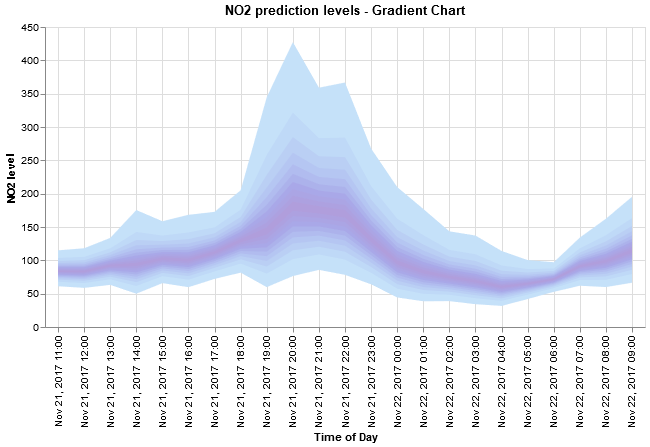
\includegraphics[width=0.4\textwidth]{gradient} 
  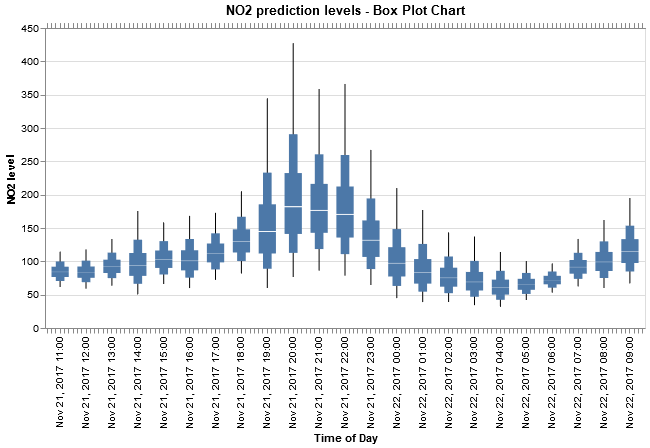
\includegraphics[width=0.4\textwidth]{boxplot}
  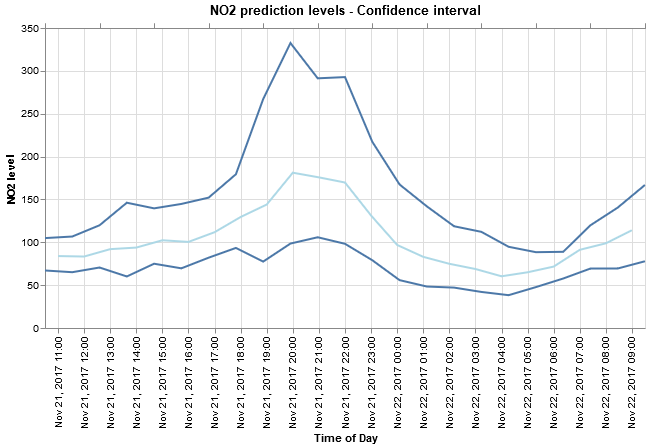
\includegraphics[width=0.4\textwidth]{ci} 
  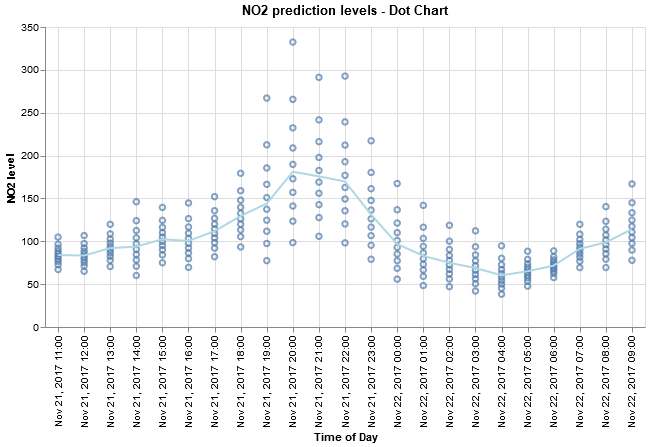
\includegraphics[width=0.4\textwidth]{dot}
  \caption{\label{figure:charts} Probabilistic Time Series Chart. 
  Top Left: Gradient Chart. Top Right: Box Plot. 
  Bottom Left: Confidence Interval. Bottom Right: Dot Chart.  }
\end{figure}

\subsection{Application: No levels forecast in Madrid}

Air quality has become a concern in recent years and lately pollution peaks have forced local authorities to take measures like cutting traffic or blocking certain city areas. Those measures are purely reactive and therefore a forecast of pollution might be preferrable as proactive measures could be taken and prevent the pollution peak before it happens.

Several stations in Madrid record the levels of NO in different parts of the city. We use a probabilistic
machine learning model to predict the levels of No in one of the stations. Instead of providing a point estimate, it provides a probability distribution at each of the prediction horizons. We represent the predictions. in a chart. This chart will be used by the authorities whenever a decision must be reached regarding the levels of pollution and preventive actions to be taken.

\section{Experimental Design}
\label{sec:exp_design}

We would like to compare 4 different types of charts displaying a probabilistic time series forecast. For this, we will evaluate how well the charts can help answering a probability question regarding the NO levels. We will request the participation of users through the Amazon Mechanical Turk website. Those users will perform a small task in exchange for a small fee (few dollars). The assigned task is a test where we measure how well can the participants read the charts. As seen in cite, we are selecting Masters Level Participants.

For each type of chart, we designed a test. Each test has a presentation part where we explain how the charts works and how it can be read and a questions part with 5 probability questions. Figure X shows the presentation part of the time series dot chart. The questions require reading the chart to estimate the probability of the NO levels inside a certain interval. We will measure for each question the error in the estimation and the time it took to answer. Inspired by the work of /cite, we are also asking at the end of the survey how difficult was reading the chart and answering the questions and how confident are they with their answers. Brenner et al. called this the load and confidence of each chart.

Figure shows the layout of one of the questions for the time series dot chart

\section{Results}
\label{sec:results}

Figure \ref{figure:errors} shows the histogram of errors for each type of chart. As we can see, the time series dot chart is clearly superior to the other charts as most of the errors are around the zero value. We will use the rank order statistic to order the performance of each type of visualization. Figure X shows the rank. We did not see an improvement in the error rate as users were answering questions.

\begin{figure}
  \centering
  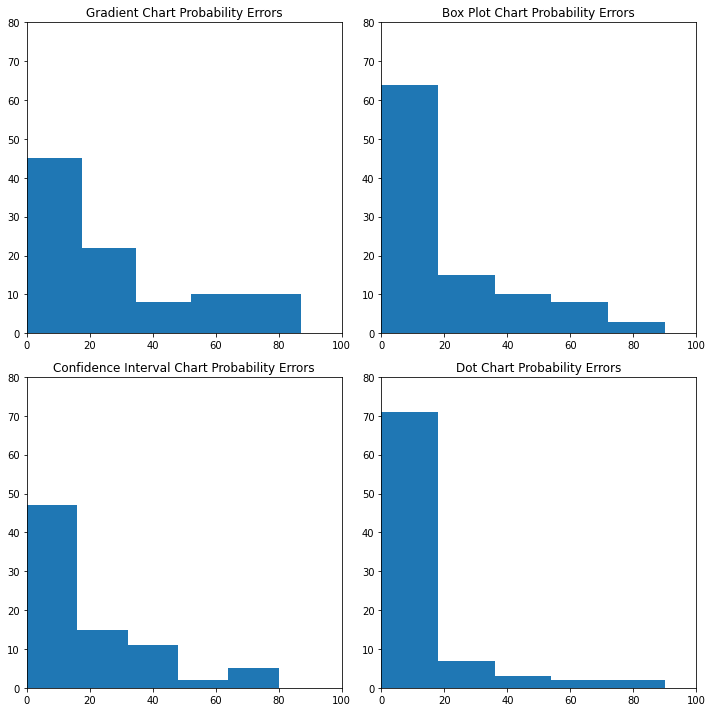
\includegraphics[width=0.6\textwidth]{probability_errors}
  \caption{\label{figure:errors}Distribution of absolute error for all questions per type of chart.}
\end{figure}

We also see in figure \ref{figure:duration} that for every chart, the time it takes to read and answer the question decreases for every question answered. We also did not see noticeable difference between the charts. However, the difficulty of reading the chart might impact this number for a higher number of questions.

\begin{figure}
  \centering
   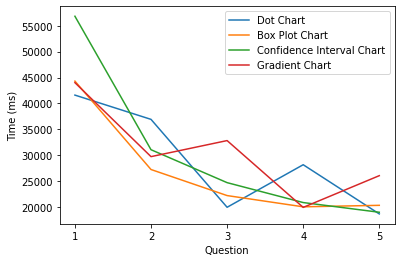
\includegraphics[width=0.6\textwidth]{duration_evo}
  \caption{\label{figure:duration} Median Time it took to answer each question for each of the types of chart.}
\end{figure}  

Confidence and load also prove the superior performance of the time series dot chart. Figure \ref{figure:confi_load} shows how the dot chart reports higher levels of confidence and lower levels of load of difficulty.

\begin{figure}
  \centering
   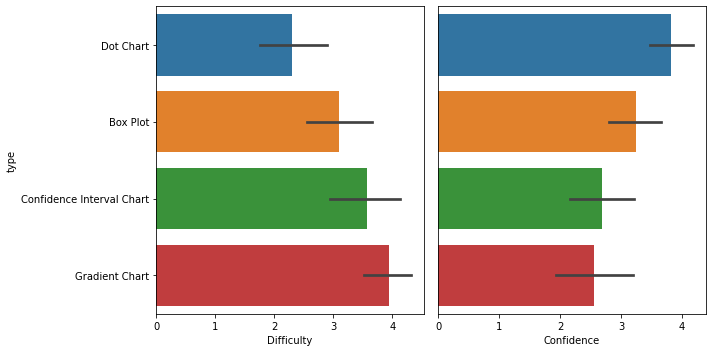
\includegraphics[width=0.5\textwidth]{confi_load}
  \caption{\label{figure:confi_load}Confidence (left) and Difficulty (right) in reading and answering the questions for each chart}
\end{figure}

We also see a lack of statistical knowledge from standard users as some users were reporting probabilities above 1, showing they do not understand the basic theory of statistics. We reported 9 users from 80 whose answers could not be used as their answers could not be applicable (probability higher than 100 o text).

\section{Conclusions}
\label{sec:concl}

\bibliography{refs}

\end{document} 

